\section{CMS und Datenbank}
\label{sec:backend}

Die Anforderungen an CMS und Datenbanken für Kiosksysteme können sehr unterschiedlich sein. 
Darüberhinaus gibt es für CMS eine große Auswahl an kommerziellen und freien Softwareprodukten.
Nach der Anforderungsanalyse aus \autoref{chap:anforderungen} muss das CMS den Anforderungen
\ref{nfa9}, \ref{nfa8} und \ref{nfa3} gerecht werden.\\

\ref{nfa3} stellt die Forderung der Multilingualität an die Oberfläche der Clientsoftware. 
Um dies zu erfüllen müssen Inhalte mehrsprachig verfügbar sein, also muss auch 
das CMS die Möglichkeit bieten Datenobjekte mehrsprachig anzulegen.\\

\ref{nfa8} stellt die Forderung der Modularität an die Software. 
Dabei spielt auch die Kopplung zwischen CMS und 
Clientapplikation eine Rolle und diese sollte möglichst gering sein. Eine geringe Kopplung
wird erreicht, wenn das CMS nicht für die Darstellung der Daten verantwortlich ist, sondern 
diese nur über eine Schnittstelle zur Verfügung stellt. CMS dieser Art besitzen also 
keine Präsentationsschicht und werden deshalb als \emph{headless} bezeichnet \cite{headless-market}.
Die Darstellung der Daten findet alleinig in der Clientapplikation statt.\\

Und schließlich fordert \ref{nfa9}, dass das CMS über das Internet erreichbar ist. 
Das CMS sollte also selbst eine Webanwendungen sein, welche auf einem über das Internet erreichbarem Server
gehostet ist.\\

All diese Anforderungen werden von vielen auf dem Markt verfügbaren CMS-Systemen erfüllt
und sind daher weniger außergewöhnlich. Beispielsweise besitzt auch das sehr verbreitete CMS \emph{Wordpress} 
standardmäßig eine REST-API, über die Daten abgefragt werden können \cite{wordpress}. Zusammen mit einem 
Plugin wie \emph{WP Headless} \cite{wordpress-headless}, welches die Präsentationsschicht von Wordpress
entfernt, kann es so ebenfalls headless betrieben werden.\todo{mehr Beispiele aufzählen} \\

\begin{figure}
    \centering
    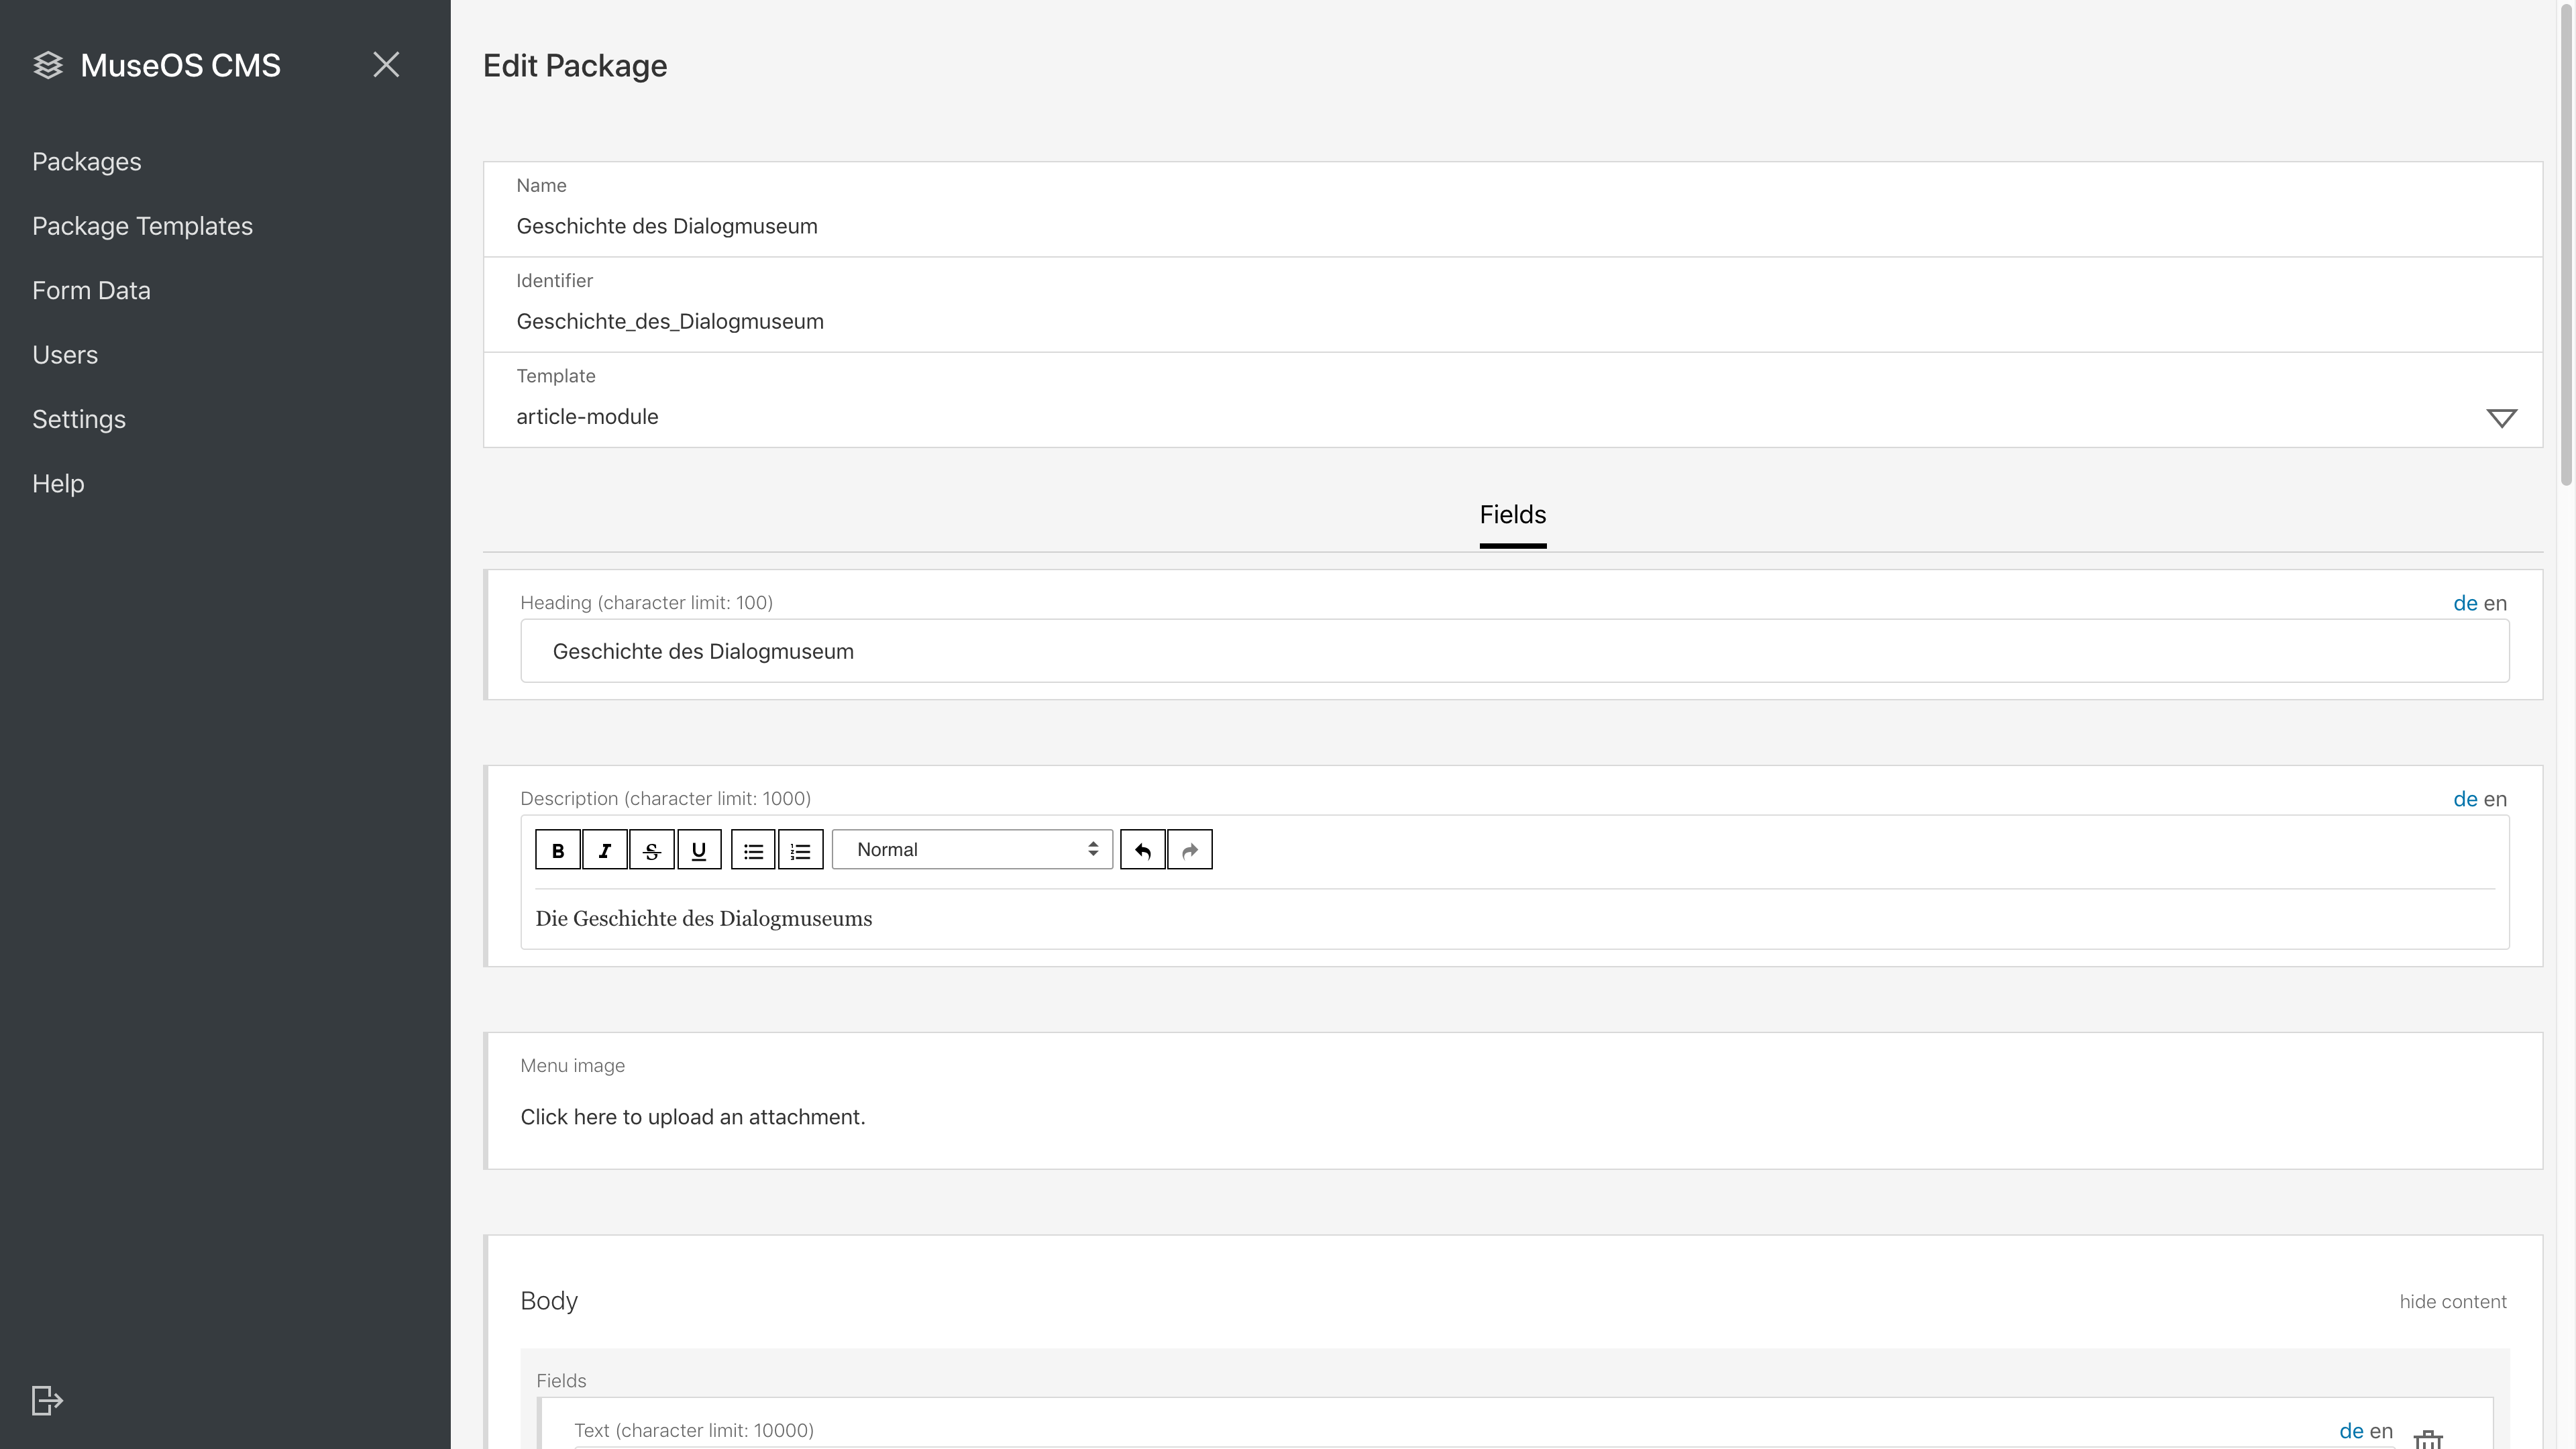
\includegraphics[width=1\textwidth]{figures/images/cms-interface.png}
    \caption{Weboberfläche des CMS}
    \label{fig:cms-interface}
\end{figure}

Für das Backend der \shst{} wurde auf ein bereits vorhandenes, von \meso{} entwickeltes,
CMS zurückgegriffen. Es wurde jedoch vom Autor dieser Arbeit
an manchen Stellen angepasst und um einige Funktionen
erweitert. Es ist in Node.js \cite{node} geschrieben und speichert die Daten in einer 
MongoDB \cite{mongo}.\\
Es handelt sich dabei um ein reines headless CMS. Es besitzt neben einer JSON-API um die Daten 
auszuliefern noch eine Upload-Schnittstelle sowie eine Schnittstelle um Formulardaten abzuspeichern
(\ref{nfa8}).\\
Die Struktur des CMS ist Template-basiert \todo{Schreibweise checken}. Administratoren können Templates 
anlegen, welche eine Datenstruktur definieren. Redakteure können dann anhand dieser Templates 
konkrete Content-Objekte erstellen, welche baumartig miteinander verknüpft werden. Templates 
werden dabei mithilfe von verschiedenen Datenfeldern gebildet. Datenfelder sind zum Beispiel
Zahlenfeld, Textfeld oder Rich-Text-Feld. Datenfelder können dabei als übersetzbare Felder angelegt
werden. Beim Erstellen eines Content-Objekts können später so verschiedene Sprachversionen
hinterlegt werden (\ref{nfa3}).\\
Das CMS ist dauerhaft bei einem Cloud-Anbieter gehostet und die Oberfläche somit über das
Internet aufrufbar (\ref{nfa9}). \autoref{fig:cms-interface} zeigt diese Oberfläche.

\todo{Screenshots vom CMS einfügen}
\todo{Links in RTF erläutern}

\iffalse
Template-basiert
Admins können Templates mit Datenstruktur erstellen
Redakteure können Objekte anhand von Templates erstellen
Sharing Station gibt Templates für Menü oder Modul
Navigationsstruktur der Oberfläche ist Baumartig - so sind auch die Daten
\fi